\documentclass{article}
%%%%%%%%%%%%%%%%%%%%%%%%%%%%%%%%%%%%%%%%%%%%%%%%%%%%%%%%%%%%%
% Lecture Specific Information to Fill Out
%%%%%%%%%%%%%%%%%%%%%%%%%%%%%%%%%%%%%%%%%%%%%%%%%%%%%%%%%%%%%
\newcommand{\LectureTitle}{L19: Shadows and Interreflections}
%\newcommand{\LectureDate}{\today}
\newcommand{\LectureDate}{March 17, 2015}
\newcommand{\LectureClassName}{CS 557}
\newcommand{\LatexerName}{Peter Henderson}
%%%%%%%%%%%%%%%%%%%%%%%%%%%%%%%%%%%%%%%%%%%%%%%%%%%%%%%%%%%%%

% Change "article" to "report" to get rid of page number on title page
\usepackage{amsmath,amsfonts,amsthm,amssymb}
\usepackage{setspace}
\usepackage{Tabbing}
\usepackage{fancyhdr}
\usepackage{lastpage}
\usepackage{extramarks}
\usepackage{chngpage}
\usepackage{soul,color}
\usepackage{graphicx,float,wrapfig}
\usepackage{afterpage}
\usepackage{abstract}
\usepackage{pgfplots}
\usepackage{caption}
\usepackage{listings}
\usepackage{minted}
\usepackage{url}

% In case you need to adjust margins:
\topmargin=-0.45in
\evensidemargin=0in
\oddsidemargin=0in
\textwidth=6.5in
\textheight=9.0in
\headsep=0.25in
\tikzstyle{cnstyle}=[domain=0:1, samples=100, ultra thick]

% Setup the header and footer
\pagestyle{fancy}
\lhead{\LatexerName}
\chead{\LectureClassName: \LectureTitle}
\rhead{\LectureDate}
\lfoot{\lastxmark}
\cfoot{}
\rfoot{Page\ \thepage\ of\ \pageref{LastPage}}
\renewcommand\headrulewidth{0.4pt}
\renewcommand\footrulewidth{0.4pt}

%%%%%%%%%%%%%%%%%%%%%%%%%%%%%%%%%%%%%%%%%%%%%%%%%%%%%%%%%%%%%
% Some tools
\newcommand{\enterTopicHeader}[1]{\nobreak\extramarks{#1}{#1 continued on next page\ldots}\nobreak
                                    \nobreak\extramarks{#1 (continued)}{#1 continued on next page\ldots}\nobreak}
\newcommand{\exitTopicHeader}[1]{\nobreak\extramarks{#1 (continued)}{#1 continued on next page\ldots}\nobreak
                                   \nobreak\extramarks{#1}{}\nobreak}

\newlength{\labelLength}
\newcommand{\labelAnswer}[2]
  {\settowidth{\labelLength}{#1}
   \addtolength{\labelLength}{0.25in}
   \changetext{}{-\labelLength}{}{}{}
   \noindent\fbox{\begin{minipage}[c]{\columnwidth}#2\end{minipage}}
   \marginpar{\fbox{#1}}

   % We put the blank space above in order to make sure this
   % \marginpar gets correctly placed.
   \changetext{}{+\labelLength}{}{}{}}

\setcounter{secnumdepth}{0}
\newcommand{\TopicName}{}
\newcounter{TopicCounter}
\newenvironment{Topic}[1][Problem \arabic{TopicCounter}]
  {\stepcounter{TopicCounter}
   \renewcommand{\TopicName}{#1}
   \section{\TopicName}
   \enterTopicHeader{\TopicName}}
  {\exitTopicHeader{\TopicName}}

\setcounter{secnumdepth}{0}
\newcommand{\ExampleSectionName}{}
\newcounter{ExampleSectionCounter}[TopicCounter]
\newenvironment{ExampleSection}[1][Example \arabic{ExampleSectionCounter}]
  {\stepcounter{ExampleSectionCounter}
   \renewcommand{\ExampleSectionName}{#1}
   \section{\ExampleSectionName}
   \enterTopicHeader{\ExampleSectionName}}
  {\exitTopicHeader{\ExampleSectionName}}

\setcounter{secnumdepth}{0}
\newcounter{ExampleBoxCounter}[TopicCounter]
\newcommand{\examplebox}[1]
  {
  % We put this space here to make sure we're disconnected from the previous
   % passage
   \stepcounter{ExampleBoxCounter}
   \noindent\fbox{\begin{minipage}[c]{\columnwidth}#1\end{minipage}}\enterTopicHeader{\ExampleSectionName}\exitTopicHeader{\ExampleSectionName}\marginpar{\fbox{\#\arabic{ExampleBoxCounter}}}
   % We put the blank space above in order to make sure this
   % \marginpar gets correctly placed.
   \vskip10pt
   }

\renewcommand{\contentsname}{{\normalsize Topics Covered}}
\renewcommand{\abstractname}{\LectureTitle\ Summary}
\renewcommand{\absnamepos}{flushleft}

\pgfplotsset{vasymptote/.style={
    before end axis/.append code={
        \draw[densely dashed] ({rel axis cs:0,0} -| {axis cs:#1,0})
        -- ({rel axis cs:0,1} -| {axis cs:#1,0});
    }
}}

%%%%%%%%%%%%%%%%%%%%%%%%%%%%%%%%%%%%%%%%%%%%%%%%%%%%%%%%%%%%%

\begin{document}
\begin{spacing}{1.1}
\newpage

% When topics are long, it may be desirable to put a \newpage or a
% \clearpage before each Topic environment
%\newpage
\begin{Topic}[Shadows \Roman{TopicCounter}]
Types of shadow: \textbf{attached} ($\vec{n} \cdot \vec{l} < 0$, a total part of the object doesn't see a light source), \textbf{cast} (relationship between surfaces).

\subsection{Blinn-Phong Model with Shadows}

Let the function $S(x) = 1$ when the light source is visible from x, and let $S(x) = 0$ when it not (i.e. shadow).

$$I(x) = S(x) \{I_l(x) k_d n(x) \cdot l(x) + I_{specular}(x)\} + I_{amb}k_a(x)$$

\subsection{Ray Tracing With Shadows}

\begin{minted}{c}
for each pixel {
	cast a ray through that pixel into the scene to find an intersection point (x,y,z)
	compute RGB ambient light component at (x,y,z)
	for each point light source{
		cast a ray from (x,y,z) to light source
		// check if light is visible, called "shadow testing"
		if light source is visible
			add RGB contribution from that light source
	}
}
\end{minted}

\subsection{Shadow Mapping}
Basic idea: instead of asking ``for each point in the scene, which lights are visible ?", we ask
``what is seen from the light source's viewpoint?"

A \textbf{shadow map} is a depth map as seen from the light source. \textit{This term is potentially confusing. A surface is seen from the light source when it is NOT in shadow.}\footnote{Haines, Eric A., and Donald P. Greenberg. ``The light buffer: A shadow-testing accelerator." 1986}

\subsection{Coordinate Systems}
Let $(x_{light}, y_{light}, z_{light})$ be continuous light source coordinates.\\
Let $(x_{shadow}, y_{shadow}, z_{shadow})$ be discrete shadow map coordinates with $z_{shadow}$ having 16 bits per pixel.\\
In both cases, assume the points have been projectively transformed, and coordinates are normalized to [0, 1] x [0, 1] x [0, 1].

\begin{center}
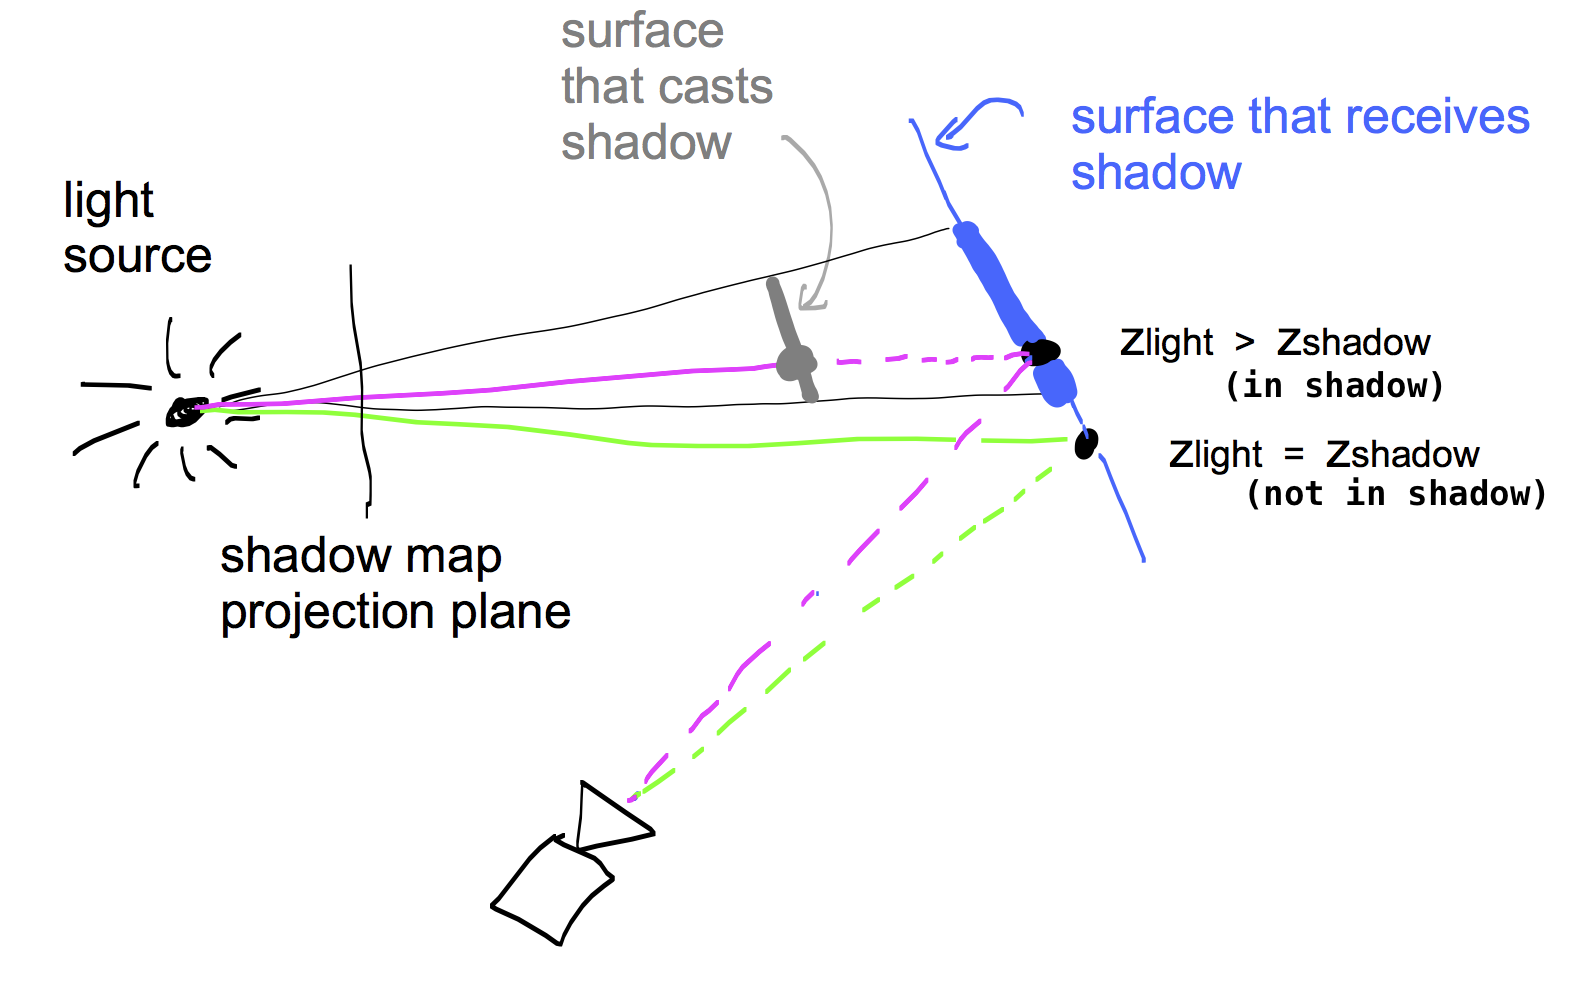
\includegraphics[scale=.3]{images/shadow_map}
\end{center}

This illustration shows perspective view, but in fact the comparisons are done in normalized coordinates (i.e. after projective transform). There are mistakes, however, because you're comparing the $z_{light}$ to $z_{shadow}$ but as we recall these are continuous vs. discrete values so cannot be equal.

\subsection{Shadow Mapping Algorithm}
\textbf{Basic Algorithm Sketch}
\begin{minted}{c}
for each camera image pixel (xp,yp) {
 find depth zp of closest visible surface // using whatever method
 transform camera coords (xp, yp, zp) to light coordinates ( xlight, ylight, zlight )
 compare zlight to zshadow( xshadow, yshadow ) to decide if 3D point is in shadow
 compute RGB
}
\end{minted}

But if you implement this, it's not going to work (because of the round off problem mentioned previously when comparing continuous to discrete points). \\
\textbf{Two Pass Algo}\\
\begin{minted}{c}
Pass 1:
	Compute only a shadow map z_shadow.
Pass 2:
	// Assume just one light source (can be generalized)
	for each camera image pixel (xp,yp) {
		find depth zp of closest visible surface
		transform (xp,yp, zp) to light coordinates (xlight, ylight, zlight)
		// to pixel positions in shadow map
		( xshadow, yshadow ) = discretize(xlight, ylight)
		if zlight > zshadow( xshadow, yshadow )
			S(xp,yp) = 0 // light source is not visible from point
		else // i.e. point in shadow
			S(xp,yp) = 1 // light source is visible from point
		calculate RGB value e.g. using Blinn-Phong model with shadow
	}
\end{minted}

\subsection{Aliasing}
What causes the aliasing? Consider the 2D xz example below.\\
$(x_{light}, z_{light})$ is on a continuous visible surface (blue curve). $(x_{shadow}, z_{shadow})$ is in the discretized shadow map (black points). The shadow condition, $z_{shadow}(x_{shadow}) < z_{light}$ , is supposed to be false because all points on the surface are visible. However, because of discretization, the condition is often true and the algorithm mistakenly concludes that some points are shadowed. To conclude that (xlight , zlight) is in shadow, in the presence of discretization, we require that a stronger condition is met:\\
$$z_{shadow}(x_{shadow}) < z_{light} - \epsilon$$
However, this can lead us to conclude that a point is not in shadow when in fact it is in shadow. When the shadow caster is on the point where the shadow gets cast, the $\epsilon$ value leads to issues.

\subsection{RealTime Rendering}
\begin{center}
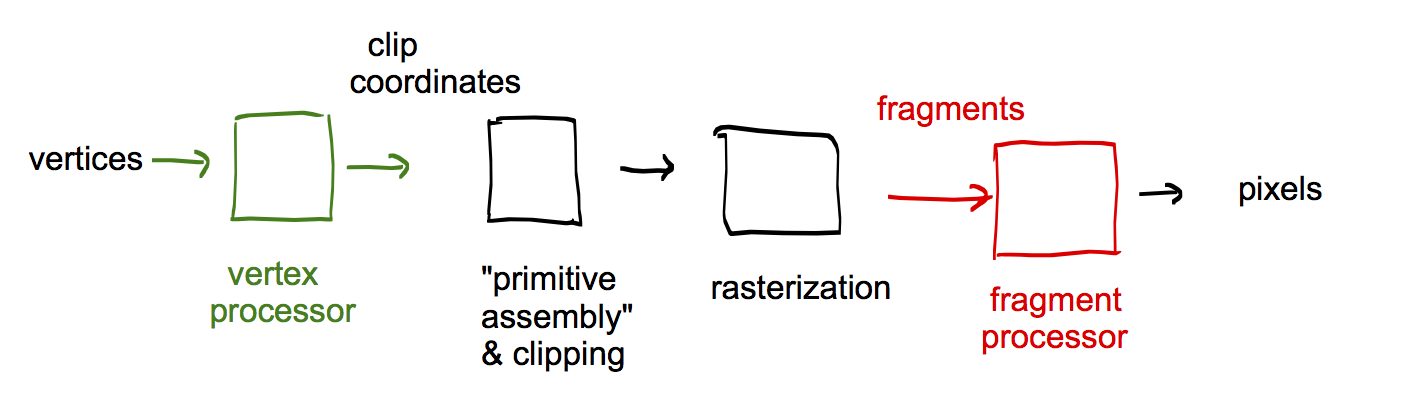
\includegraphics[scale=.34]{images/shadow_pipeline}
\end{center}

\subsubsection{Pass 1: Compute Shadow Map}
\textbf{vertex shader}: transform vertices to light coordinates $( x_{light}, y_{light}, z_{light} )$\\
\textbf{rasterizer}: for each light source pixel $( x_{shadow}, y_{shadow} )$ find depth $z_{shadow}$ of closest surface\\
\textbf{fragment shader:} store depths as a texture $z_{shadow}( x_{shadow}, y_{shadow} )$
\subsubsection{Pass 2: Make RGB Image With Shadows}
\textbf{vertex shader}: transform vertices to light coordinates $( x_{light}, y_{light}, z_{light} )$ (like in pass 1)\\
\textbf{rasterizer}: generate fragments (each fragment needs $(x_p, y_p ), n, z, x_{shadow}, y_{shadow}, z_{light}$)\\
\textit{The rasterizer does not have access to the shadow map computed in the first pass. The fragment shader (below) has access to it.}\\
\textbf{fragment shader}:\\
\begin{minted}{c}
if zshadow( xshadow, yshadow ) + EPS_VALUE < zlight
	compute RGB using ambient only // in shadow
else
	compute RGB using Blinn-Phong // not in shadow
\end{minted}

You have to look up the $z_{shadow}$ value from the previously stored texture from the first pass.

\subsection{Ambient Occlusion}
How to handle ``diffuse lighting'' (i.e. outdoors on an overcast day, uniformly illuminated indoor scene like classroom, factory, office, retail store)?

\subsubsection{Visibility of the Sky}
\begin{center}
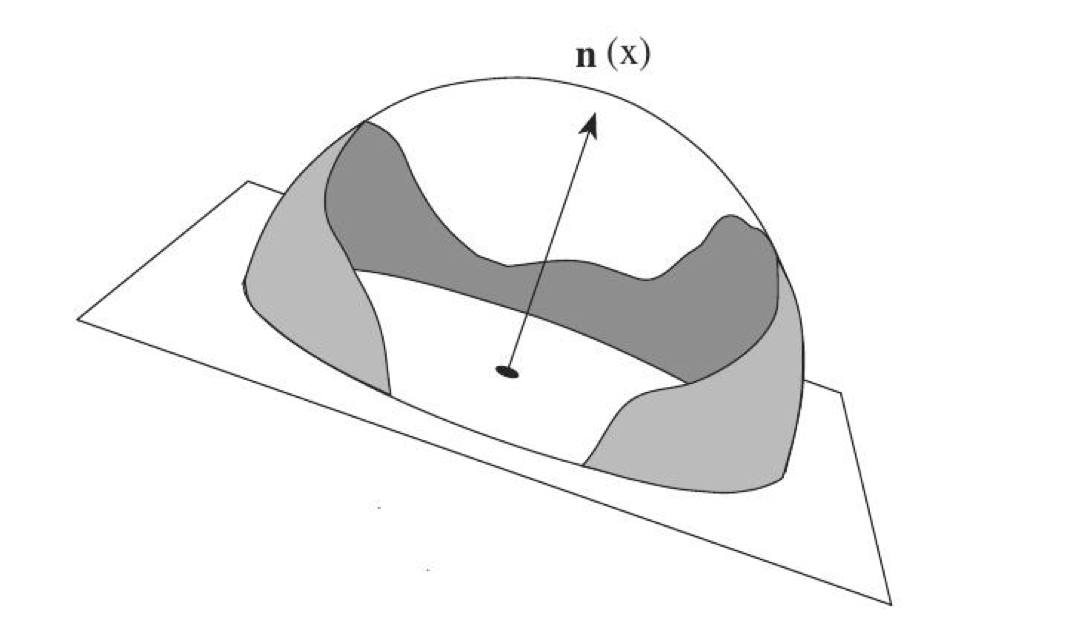
\includegraphics[scale=.34]{images/hem}
\end{center}

In the above image you have a hemisphere of directions from a point on a plane from which you can receive light (dark regions represent no light getting through). So we have to add up over all directions where the sky is visible, the light contribution. Where $S(x,l)$ is a sky source function when it is not uniform as above.
$$I_{diffuse}(x)= \int_{S(x,l)} n(x) \cdot l \delta l$$

\begin{center}
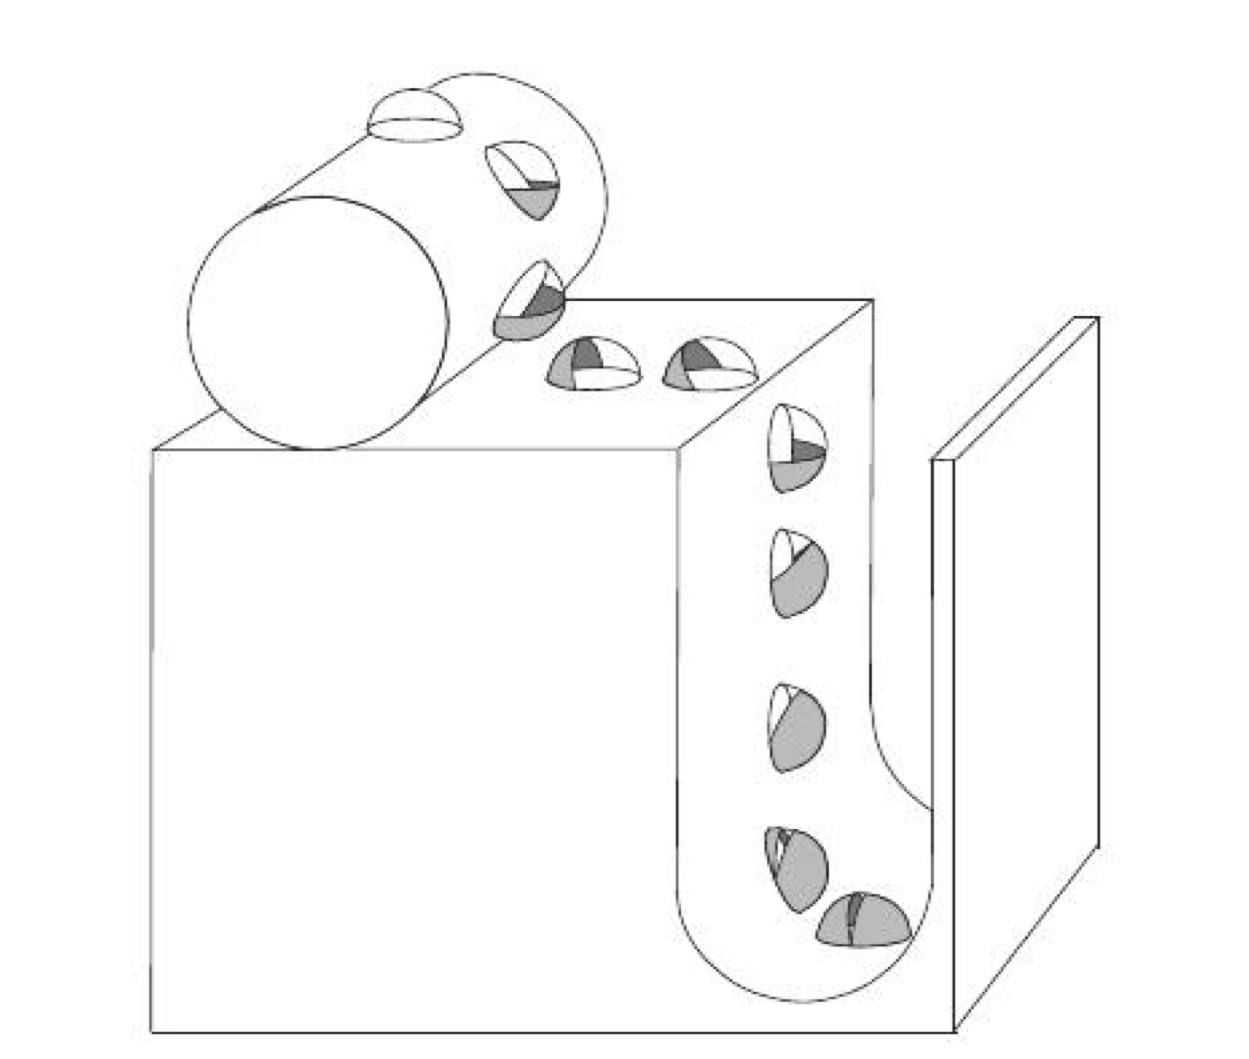
\includegraphics[scale=.34]{images/skysphere}
\end{center}

As can be seen above this sky source function is variable across different points of the surfaces.

\textbf{One possible solution is as follows.}

Assume that: (1) the light source is a uniform distant hemisphere, (2) the fraction of the source is determined only by the surface normal.

$$ I_{diffuse}(x) = \frac{1 + n(x) \cdot \hat{y}}{2}$$

What are the differences of this model and a sunny day scenario? Key limitation: the model on the previous slide cannot account for cast shadows, e.g. illumination variations along the ground plane or along the planar side of the gully, since the normal is constant on a plane.

\textbf{Another solution uses Ray Tracing}

\begin{minted}{c}
for each pixel in the image {
	cast a ray through the scene point to find the nearest surface (x,y,z)
	shoot out rays from (x, y, z) into the hemisphere and check which of them reach the "sky"
		//i.e. infinity or some finite distance
	add up environment contribution of rays that reach the "sky"
		// you could have a non-uniform sky
}
\end{minted}

\textbf{Another solution is ambient occlusion}\footnote{Zhukov, Sergey, Andrei Iones, and Grigorij Kronin. "An ambient light illumination model." 1998}

\begin{minted}{c}
// precompute
for each vertex x {
	shoot out rays into the hemisphere
	calculate the fraction of rays, S(x) in [0, 1], that reach the "sky"
	// S(x) is an attribute of x, along with n and material
	// If you are willing to use more memory, then store the
	// a boolean map S(x, l), where l is direction of light
	// See Exercises.
}
// We say that S(x) is "baked" into the surface.
\end{minted}

Ambient occlusion can replace $n(x) \cdot l$ term in more general Blinn-Phong model instance to simply $S(x)$.

So \textit{how to do ambient occlusion with indoor scenes?} For each vertex, compute S(x) in [0, 1] by considering only surfaces within some distance of x. So anything beyond x you assume is sky.

\subsection{Interreflections}

Points don't just receive light from sources, but also from reflections off of other objects which results in some color bleeding. (Cornell Box, 1984)

Computing interreflections is a linear algebra problem (indirect component is due to bouncing off of other surfaces):
$$I(x) = I_{direct}(x) + I_{indirect}(x)$$

But $I_{indirect}(x)$ is the sum of $I(y)$ for points y that are visible from x. Thus,
$$I(x) = I_{direct}(x) + \sum_y F(x,y) I(y)$$
where $F(x,y)$ depends on: (1) distance between x and y, (2) n(x) and n(y), (3) whether x and y see each other. However, these are huge vectors and matrices. so researchers have created many clever numerical methods for solving this. These interreflection methods ("global illumination") can now produce photorealistic images of complex scenes. Solutions are still expensive though...

\end{Topic}

\end{spacing}
\end{document}